\subsection{Maßangaben und Variation Mining}

\newcommand{\Gen}{\ensuremath{_{\mathsf{Gen}}}}
\newcommand{\Acc}{\ensuremath{_{\mathsf{Acc}}}}


\begin{frame}
	{Schäfer (wird 2016 eingereicht)}
	\scalebox{0.85}{\begin{minipage}{1.2\textwidth}
	\begin{exe}
		\ex\gll Wir trinken eine Flasche [des {Weines]\Gen} {\slash} *[den Wein]\Acc.\\
			we drink a bottle [the wine]{\Gen} {\slash} \hspaceThis{*}[the wine]\\
			\glt {\it We drink a bottle of the wine.}
		\ex\gll Wir trinken eine Flasche {*Weines\Gen} {\slash} Wein\Acc.\\
			we drink a bottle \hspaceThis{*}wine {\slash} wine\\
			\glt {\it We drink a bottle of wine.}
		\ex\gll Wir trinken eine Flasche [leckeren {Weines]\Gen} {\slash} [leckeren Wein]\Acc.\\
			we drink a bottle tasty wine / tasty wine\\
			\glt {\it We drink a bottle of tasty wine.}
	\end{exe}
	\end{minipage}}
\end{frame}

\begin{frame}
	{German measure NPs}
	\begin{itemize}
		\item measure phrases in the broad sense
		\item {$[N_{measure}\ Det\ (AP)\ N_{kind}]$}: case of $N_{kind}$ always genitive
		\item {$[N_{measure}\ N_{kind}]$}: always case identity
		\item {$[N_{measure}\ AP\ N_{kind}]$}: genitive or case identity 
	\end{itemize}
\end{frame}

%\begin{frame}
%	{Case syncretism in the feminine}
%	\begin{itemize}
%		\item feminine NPs: syncretisms of nom\slash acc and dat\slash gen
%		\item nom\slash acc: \textit{(eine\slash die) frische Sahne}
%		\item dat\slash gen: \textit{(einer\slash der) frischen Sahne\slash frischer Sahne}
%		\item decision not between case-identity and genitive construction\\
%			but case-identity and obliqueness-drop construction
%	\end{itemize}
%\end{frame}
%
%\begin{frame}
%	{Descriptive gap}
%	\begin{itemize}
%		\item descriptions in grammars\\(e.g., Eisenberg 2013, Engel 2009)
%		\item genitive construction: \textit{partitive genitive}
%		\item case-identity construction: \textit{narrow apposition}
%	\end{itemize}
%\end{frame}

%\begin{frame}
%	{Unambiguous structures (semi-hypothetical account)}
%	\centering
%	\scalebox{0.8}{\begin{minipage}{0.5\textwidth}\centering
%	\begin{forest}
%		[DP [D[eine]] [NP [N[Flasche]] [NP[Wein]] ]] ]]
%	\end{forest}
%	\end{minipage}}
%	\scalebox{0.8}{\begin{minipage}{0.5\textwidth}\centering
%	\begin{forest}
%		[DP [D[eine]] [NP [N[Flasche]] [DP [D[des]] [NP [AP[guten]] [N[Weines]] ] ]]]
%	\end{forest}
%	\end{minipage}}
%\end{frame}
%
%\begin{frame}
%	{Ambiguous structures (semi-hypothetical account)}
%	\centering
%	\scalebox{0.8}{\begin{minipage}{0.5\textwidth}\centering
%	\begin{forest}
%		[DP [D[eine]] [NP [N[Flasche]] [NP [AP[guter]] [N[Wein]]] ]] ]]
%	\end{forest}
%	\end{minipage}}
%	\scalebox{0.8}{\begin{minipage}{0.5\textwidth}\centering
%	\begin{forest}
%		[DP [D[eine]] [NP [N[Flasche]] [DP [D[guten]] [NP [Weines]] ] ]]
%	\end{forest}
%	\end{minipage}}
%\end{frame}
%
%\begin{frame}
%	{Sense and syntacticality}
%	\begin{itemize}
%		\item configurational approaches like that in\\Bhatt (1990), Gallmann \& Lindauer (1994), etc.
%		\item interestingly: often, one alternative considered \textit{ungrammatical}
%		\item sometimes additional \textit{QP} level
%		\item Gallmann (1990): single structure for both constructions
%		\item long-winded \textit{proofs}, that measure noun is the higher head (Löbel 1990, Bhatt 1990)
%		\item ... trivial, because of simple agreement facts
%	\end{itemize}
%\end{frame}
%
%\begin{frame}
%	{"The rich literature on partitives"}
%	\footnotesize
%	Partitives\slash Pseudo-partitives\slash Partitive Constraint
%	\begin{itemize}
%		\item partitives: embedded NP is definite = \textit{Partitive Constraint}\\
%			(e.\,g., Jackendoff 1977, Ladusaw 1982, Selkrik 1977, Vos 1999)
%		\item not even true for German \textit{partitive genitive} construction
%		\item German constructions: pseudo-partitives, if anything
%		\item Anttila \& Fong (2001): refined PC (\textit{quantificational determinacy})\\
%			plus some allegedly universal syntactic constraints (\textit{syntactic OCP})\\
%			to account for a highly non-similar alternation in Finnish
%		\item Eschenbach (1991) on German measure constructions:\\
%			more refined semantics, again irrelevant for our purposes
%	\end{itemize}
%\end{frame}
%
%\begin{frame}
%	{To sum up\ldots}
%	\begin{itemize}
%		\item no relevant insight from configurational approaches
%		\item no help from semantics of measurement\slash partitivity
%		\vspace{0.5cm}
%		\item \alert{no strong theoretical hypotheses\\about what drives the alternation}
%	\end{itemize}
%\end{frame}
%
%\begin{frame}
%	{Hentschel (2003)}
%	\begin{itemize}
%		\item questionnaire study
%		\item descriptive, no theoretical approach
%		\item results:
%			\begin{enumerate}
%				\item overall tendency for case identity
%				\item genitive preferred with plural nouns
%				\item verb-governed accusative: identity preferred
%			\end{enumerate}
%	\end{itemize}
%\end{frame}
%
%\subsection{Corpus study}
%
%\subsubsection{General research paradigm}

\begin{frame}
	{Alternations}
	\begin{itemize}
		\item \textit{alternations}
			\begin{itemize}
				\item competing constructions, given contexts\slash lexical choices
				\item competing items, given constructions
			\end{itemize}
		\item established paradigm: alternations as neither fully random\\
			nor controlled by discrete (even single) factors
		\item cognitively motivated: item-specific and\slash or context-specific\\
			influences on the probabilities of choices
		\item e.g., Gries (2003), Gries \& Stefanowitsch (2003 et alibi), Bresnan et al. (2007), Arppe (2009), Nesset \& Janda (2010), Divjak \& Arppe (2013), Bart \& Kapatsinski (2014 aop)
	\end{itemize}
\end{frame}

%\subsubsection{Sample(s)}
%
%\begin{frame}
%	{2012 sample}
%	\begin{itemize}
%		\item DEWAC (Baroni et al. 2009)
%		\item 30 intuitively chosen mass nouns (10 per gender)
%		\item only mass nouns (singular) 
%		\item search for sequences [N A specific-mass-noun]
%		\item filter by hand, annotate for case of measure noun
%		\item 687 masculine, 1007 neuter, 421 feminine NPs
%		\item because of low frequency of genitives,\\samples were stratified: 50\% for each level of response
%	\end{itemize}
%\end{frame}
%
%\begin{frame}
%	{2015 sample}
%	\begin{itemize}
%		\item corpus: DECOW14A (Schäfer \& Bildhauer 2012\ldots), 20 GT
%		\item again: only mass nouns (singular) 
%		\item bootstrap process:
%			\begin{enumerate}
%				\item manually extract 100 most frequent mass nouns
%				\item search pattern [N D A* N mass-noun]
%				\item manually extract the 20 most frequent measure nouns\\for each mass noun
%				\item query combinations [measure-noun A mass-noun]
%			\end{enumerate}
%		\item final sample (after filtering\slash cleaning):\\
%			4172 masculine\slash neuter, 1114 feminine
%		\item as opposed to DEWAC sample, DECOW14A sample covers\\
%			all frequent combinations of measure and mass nouns
%	\end{itemize}
%\end{frame}

%\subsubsection{GLMs for DEWAC dataset}

%\begin{frame}
%	{DEWAC: Masculine\slash Neuter}
%  \centering
%  \scalebox{0.8}{
%  \begin{tabular}{lrrcp{1cm}rrc}
%    \multicolumn{1}{c}{} & \multicolumn{3}{c}{\textbf{Masculine}} && \multicolumn{3}{c}{\textbf{Neuter}} \\
%    \hline
%    \textbf{Regressor} & \textbf{Coeff.} & \textbf{OR} & \textbf{Sign.} && \textbf{Coeff.} & \textbf{OR} & \textbf{Sign.} \\
%    \hline
%    \hline
%    \textsc{(Intercept)} & -1.95 & 0.14 & *** && -3.37 &  0.03 & *** \\
%    \textsc{MeasurecaseNom}   &  0.31 & 1.37 &   . && -0.01 &  0.99 &     \\
%    \textsc{MeasurecaseDat}   &  0.31 & 1.37 &   * &&  0.92 &  2.50 & *** \\
%    \textsc{Measurenoundefinite1}      &  1.47 & 4.36 & *** &&  2.67 & 14.48 & *** \\
%    \textsc{Kindfreq}    &  0.03 & 1.03 & *** &&  0.82 &  2.27 & *** \\
%    \textsc{Measureabbreviated1}     & -3.05 & 0.05 & *** && -4.92 &  0.01 & *** \\
%    \hline
%  \end{tabular}}\\
%  \vspace{0.5cm}
%	\footnotesize predicting \textsc{genitive construction}; model selection by step-down; internal and 10-fold cross validation accuracy is $78.01\%$ for masculine, $75.65\%$ for neuter; Nagelkerke's $R^2=0.22$ for masculine, $R^2=0.29$ for neuter; dispersion $\hat\phi=0.99$ for masculine, $\hat\phi=0.95$ for neuter
%\end{frame}
%
%\begin{frame}
%	{DEWAC: Feminine}
%  \centering
%  \scalebox{0.75}{
%  \begin{tabular}{lrrc}
%    \hline
%    \textbf{Regressor} & \textbf{Coeff.} & \textbf{OR} & \textbf{Sign.} \\
%    \hline
%    \hline
%    \textsc{(Intercept)} &  4.08 & 59.41 & *** \\
%    \textsc{MeasurecaseAcc}   & -0.16 &  0.85 &     \\
%    \textsc{MeasurecaseDat}      & -2.33 &  0.10 &   * \\
%    \textsc{Kindfreq}    & -2.00 &  0.14 & *** \\
%    \textsc{Measureabbreviated1}     &  3.65 & 38.38 & *** \\
%    \hline
%  \end{tabular}}\\
%  \vspace{0.5cm}
%	\footnotesize predicting \textsc{case agreement}; model selection by step-down; internal and 10-fold cross validation accuracy is $80.71\%$; Nagelkerke's $R^2=0.62$, dispersion is $\hat{\phi}=0.87$
%\end{frame}

%\subsubsection{GLMs from DECOW14 dataset}

\begin{frame}
	{DECOW14A model summary: masculine and neuter}
	\centering
	\scalebox{0.5}{
	\begin{tabular}{lrrrrrc}
	\hline
                   &  Estimate& OR & Std. Error& z value& Pr(>|z|)&    \\
	\hline
	\hline
		(Intercept)        & -12.36736& 0.0000 &  0.99790& -12.393&  < 2e-16& ***\\
		MeasurecaseAcc     &   0.03406& 1.0346 &  0.11721&   0.291& 0.771352&    \\
		MeasurecaseDat     &   0.49126& 1.6343 &  0.13569&   3.621& 0.000294& ***\\
		Kindlength         &   0.61327& 1.8464 &  0.03434&  17.859&  < 2e-16& ***\\
		KindfinalclassFric &  -0.04110& 0.9597 &  0.23217&  -0.177& 0.859490&    \\
		KindfinalclassRvo  &  -0.07985& 0.9232 &  0.22898&  -0.349& 0.727293&    \\
		KindfinalclassPlos &   0.52423& 1.6891 &  0.22652&   2.314& 0.020651& *  \\
		KindfinalclassLiq  &   0.85280& 2.3461 &  0.24504&   3.480& 0.000501& ***\\
		KindfinalclassNas  &   0.77421& 2.1688 &  0.24397&   3.173& 0.001507& ** \\
		Kindedible0        &   0.75699& 2.1318 &  0.12396&   6.106& 1.02e-09& ***\\
		Kindfreq           &   1.92525& 6.8568 &  0.16232&  11.861&  < 2e-16& ***\\
		MeasuregenderMasc  &   0.01090& 1.0109 &  0.15411&   0.071& 0.943634&    \\
		MeasuregenderFem   &   0.35432& 1.4252 &  0.13988&   2.533& 0.011308& *  \\
		MeasurenumberPl    &   0.86330& 2.3709 &  0.14906&   5.792& 6.97e-09& ***\\
		Measureabbreviated0&   1.53688& 4.6500 &  0.32499&   4.729& 2.26e-06& ***\\
		Measurelength      &  -0.12810& 0.8797 &  0.03397&  -3.771& 0.000163& ***\\
		Measurefreq        &  -0.58232& 0.5585 &  0.09269&  -6.282& 3.33e-10& ***\\
		Minus1posP         &   1.18411& 3.2677 &  0.21357&   5.544& 2.95e-08& ***\\
		Minus1posN         &   0.23117& 1.2600 &  0.26573&   0.870& 0.384328&    \\
		Minus1posA         &   1.86418& 6.4506 &  0.14891&  12.518&  < 2e-16& ***\\
		Minus1posO         &   2.04921& 7.7617 &  0.38346&   5.344& 9.09e-08& ***\\
		Genitives          &  -0.32547& 0.7221 &  0.02732& -11.913&  < 2e-16& ***\\
		Badness            &  -0.09064& 0.9133 &  0.02613&  -3.468& 0.000524& ***\\
	\hline
	\end{tabular}
	}
\end{frame}
%
%\begin{frame}
%	{DECOW14A model evaluation: masculine and neuter}
%	\centering
%	\begin{tabular}{llll}
%		Sample size & n &=&  4172 \\
%		Nagelkerke  & $R^2$ &=&  0.431 \\
%		Dispersion  & $\phi$ &=&  0.894 \\
%		LR Test     & LR &=&  1257.841 (df =  22, p =  0)\\
%		10-CV       & $\Delta$ &=&  0.09994593 \\
%		Baseline    & $\epsilon$ &=&  0.1744966 \\
%		Reduction   & pre &=&  0.4272329 \\
%	\end{tabular}
%\end{frame}
%
%\begin{frame}
%	{DECOW14A variance inflation: masculine and neuter}
%	Dropped for extreme collinearity:
%	\vspace{1cm}
%	\begin{enumerate}
%		\item semantics of mass noun: \textit{consistency}
%		\item semantics of mass noun: \textit{origin}
%		\item semantics of mass noun: \textit{artefact}
%		\item semantics of measure noun: \textit{semantic class}
%	\end{enumerate}
%\end{frame}
%
%\begin{frame}
%	{DECOW14A variance inflation: masculine and neuter}
%	\centering
%	\scalebox{0.8}{
%	\begin{tabular}{lrrr}
%	\hline
%		                  &     $GVIF$& $Df$& $GVIF^(1/(2*Df))$\\
%	\hline
%	\hline
%		Measurecase       & 1.068292&  2&        1.016652\\
%		Kindlength        & 1.609944&  1&        1.268836\\
%		Kindfinalclass    & 2.250817&  5&        1.084511\\
%		Kindedible        & 1.465327&  1&        1.210507\\
%		Kindfreq          & 1.338470&  1&        1.156923\\
%		Measuregender     & 1.596935&  2&        1.124144\\
%		Measurenumber     & 1.626972&  1&        1.275528\\
%		Measureabbreviated& 1.355320&  1&        1.164182\\
%		Measurelength     & 1.974751&  1&        1.405258\\
%		Measurefreq       & 1.740086&  1&        1.319123\\
%		Minus1pos         & 1.787250&  4&        1.075284\\
%		Genitives         & 1.121494&  1&        1.059006\\
%		Badness           & 1.039426&  1&        1.019523\\
%	\hline
%	\end{tabular}
%	}
%\end{frame}
%
%

\begin{frame}
	{DECOW14A model summary: feminine}
	\centering
	\scalebox{0.7}{
	\begin{tabular}{lrrrrrc}
	\hline
                   &  Estimate& OR &Std. Error& z value& Pr(>|z|)&    \\
	\hline
	\hline
		(Intercept)      & -3.26446 &  0.0382&  1.00948&  -3.234&  0.00122& ** \\
		Kindedible0      &  1.38772 &  4.0057&  0.18586&   7.467& 8.23e-14& ***\\
		MeasuregenderMasc&  0.98742 &  2.6842&  0.22957&   4.301& 1.70e-05& ***\\
		MeasuregenderFem &  0.46838 &  1.5973&  0.21722&   2.156&  0.03107& *  \\
		MeasurenumberPl  &  1.50316 &  4.4958&  0.29577&   5.082& 3.73e-07& ***\\
		Measurelength    & -0.30782 &  0.7350&  0.06044&  -5.093& 3.52e-07& ***\\
		Measurefreq      & -0.46196 &  0.6300&  0.15652&  -2.951&  0.00316& ** \\
		Minus1posP       &  1.90609 &  6.7267&  0.39414&   4.836& 1.32e-06& ***\\
		Minus1posN       &  0.68847 &  1.9906&  0.59486&   1.157&  0.24712&    \\
		Minus1posA       &  3.06176 & 21.3650&  0.28243&  10.841&  < 2e-16& ***\\
		Minus1posO       &  3.09771 & 22.1472&  0.55616&   5.570& 2.55e-08& ***\\
		Matchlength      &  0.17986 &  1.1970&  0.02229&   8.069& 7.09e-16& ***\\
		Genitives        & -0.29002 &  0.7482&  0.04288&  -6.764& 1.34e-11& ***\\
	\hline
	\end{tabular}
	}
\end{frame}
%
%\begin{frame}
%	{DECOW14A model evaluation: feminine}
%	\centering
%	\begin{tabular}{llll}
%		Sample size&  n& = & 1114 \\
%		Nagelkerke & $R^2$& = & 0.491 \\
%		Dispersion &  $\phi$& = & 1.053 \\
%		LR Test    & LR& = & 505.8554 (df =  12,    p =  0)\\
%		10-CV      &  $\Delta$& = & 0.151722 \\
%		Baseline   &  $\epsilon$& = & 0.4147217 \\
%		Reduction  &pre& = & 0.6341595 \\
%	\end{tabular}
%\end{frame}
%
%\begin{frame}
%	{DECOW14A variance inflation: feminine}
%	\centering
%	\scalebox{0.8}{
%	\begin{tabular}{lrrr}
%	\hline
%		                  &     $GVIF$& $Df$& $GVIF^(1/(2*Df))$\\
%	\hline
%	\hline
%		Kindedible   & 1.209434 & 1 &       1.099743\\
%		Measuregender& 1.780486 & 2 &       1.155140\\
%		Measurenumber& 1.657590 & 1 &       1.287474\\
%		Measurelength& 2.279081 & 1 &       1.509663\\
%		Measurefreq  & 2.120574 & 1 &       1.456219\\
%		Minus1pos    & 1.766196 & 4 &       1.073692\\
%		Matchlength  & 1.484503 & 1 &       1.218402\\
%		Genitives    & 1.101343 & 1 &       1.049449\\
%
%	\hline
%	\end{tabular}
%	}
%\end{frame}
%
%\begin{frame}
%	{A note on random effects}
%	\begin{itemize}
%		\item the mass noun lemma as a random effect was significant\\for DEWAC data
%		\item fixed effects \alert{not} masked by RE
%		\item slight increase in accuracy and $R^2$
%		\item for DECOW data: problems with model estimation\slash evaluation
%		\item \textit{speaker}, \textit{genre} not available (no meta data)
%		\item current work on COW might improve that
%	\end{itemize}
%\end{frame}

%\subsubsection{Multimodel approach for DECOW14 dataset}

\begin{frame}
	{Multimodel inference}
	\begin{itemize}
		\item some of problems with stepwise regression:
			\begin{enumerate}
				\item likely incorrect fiction of availability of a best model\\
					approximating absolute truth
				\item spurious significances\\
					\alert{especially with large samples}
				\item \textit{data dredging} without strong\\
					theoretically motivated hypotheses
			\end{enumerate}
		\item solution: consider some or even many good models
		\item model weighting by information criterion like AIC(c), BIC(c)
		\item find and average \textit{important} coefficients across models
		\item Burnham \& Anderson (2002), in linguistics:\\Kuperman \& Bresnan (2012), Bart \& Kapatsinski (2014 aop)
	\end{itemize}
\end{frame}

\begin{frame}
	{Under the circumstances...}
	\begin{itemize}
		\item We don't have strong hypotheses.
		\item But we do have large samples.
		\item Sounds like a case for MMI.
	\end{itemize}
\end{frame}

\begin{frame}
	{Multimodel averaging: masculine and neuter}
	\centering
	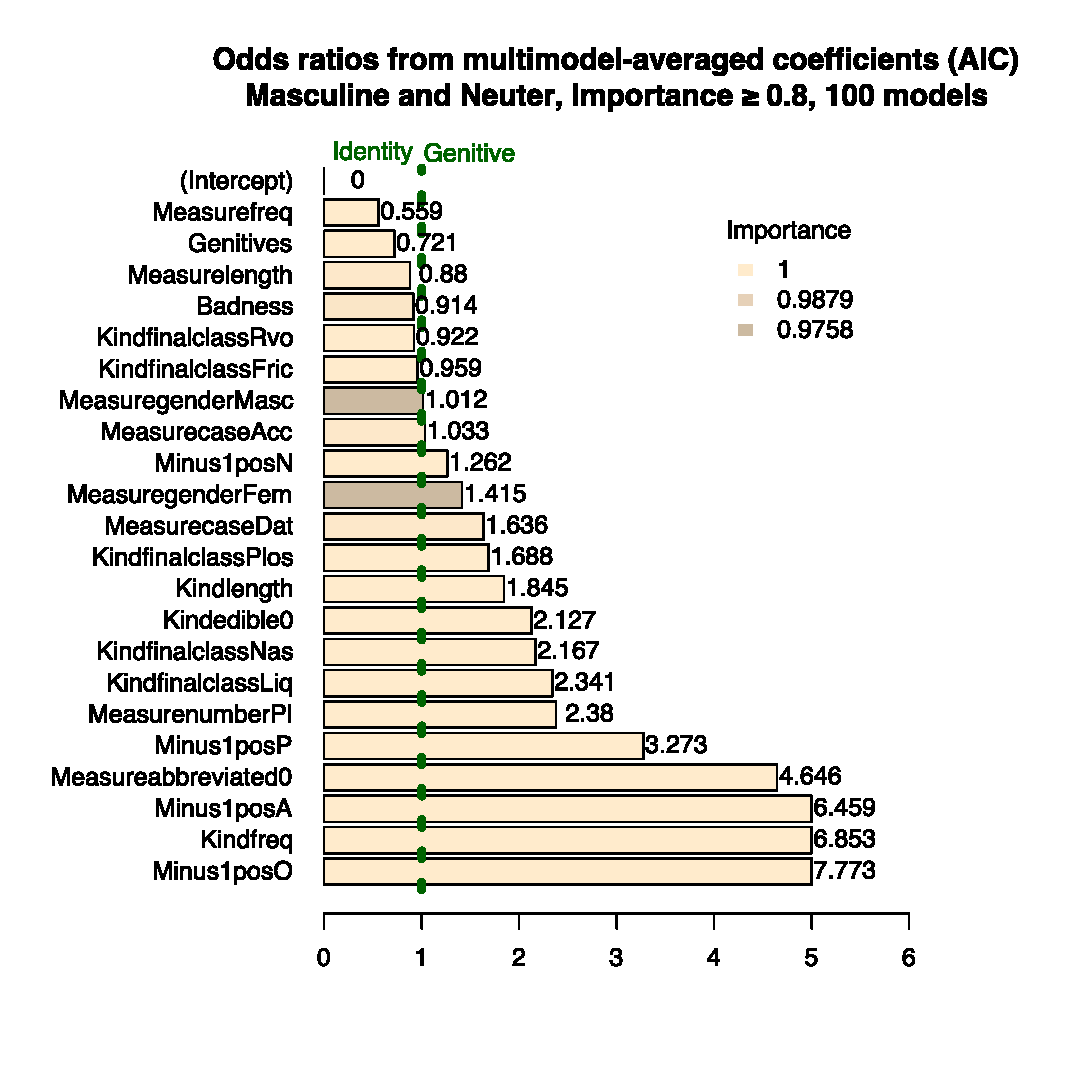
\includegraphics[height=0.8\textheight]{mn_aic_multi}\\
	\tiny genetic algorithm, search through full model space without interactions and random effects
\end{frame}

\begin{frame}
	{Multimodel averaging: feminine}
	\centering
	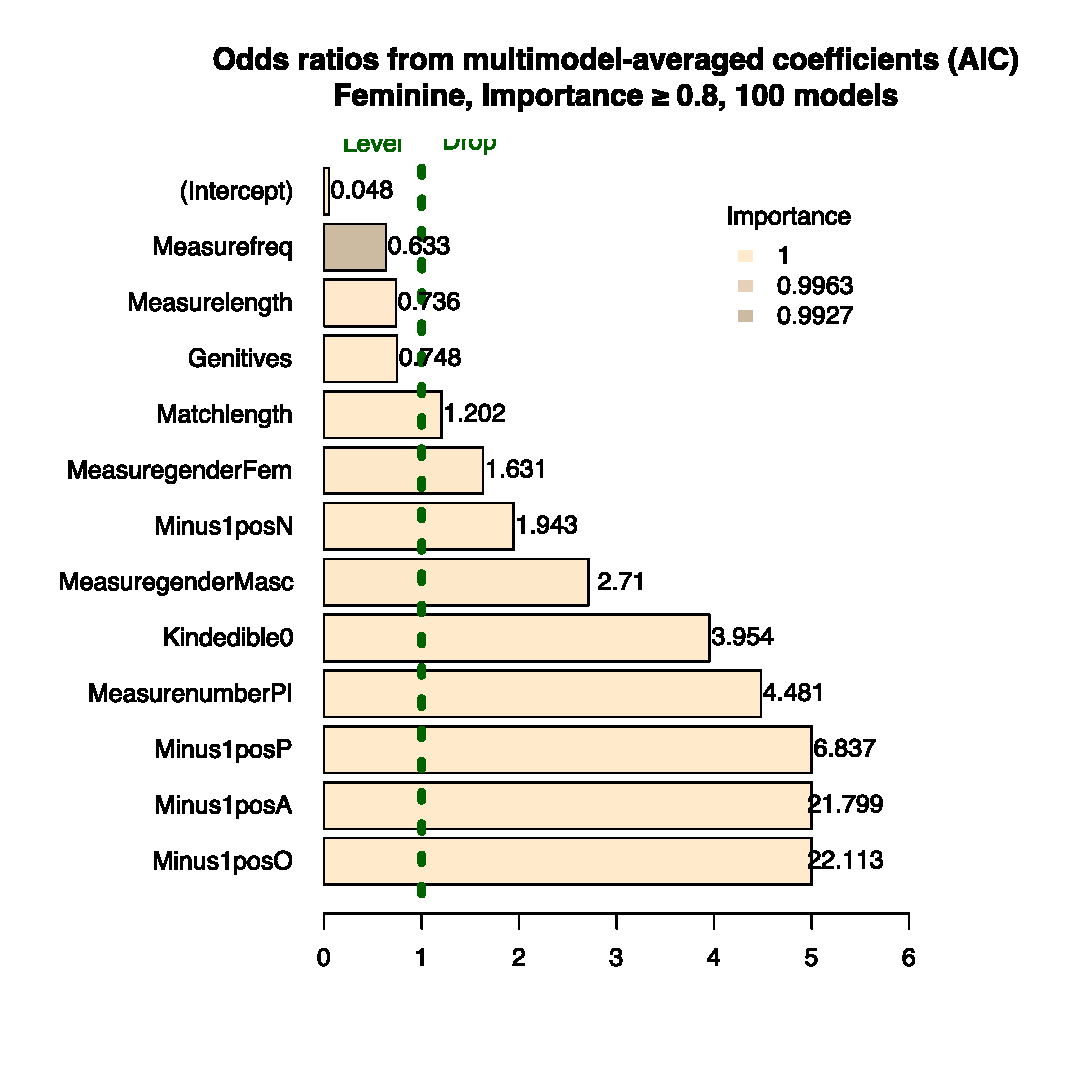
\includegraphics[height=0.8\textheight]{fem_aic_multi}\\
	\tiny genetic algorithm, search through full model space without interactions and random effects
\end{frame}

%\subsubsection{AIC and BIC}
%
%\begin{frame}
%	{Which IC to use: masculine and neuter}
%	\centering
%	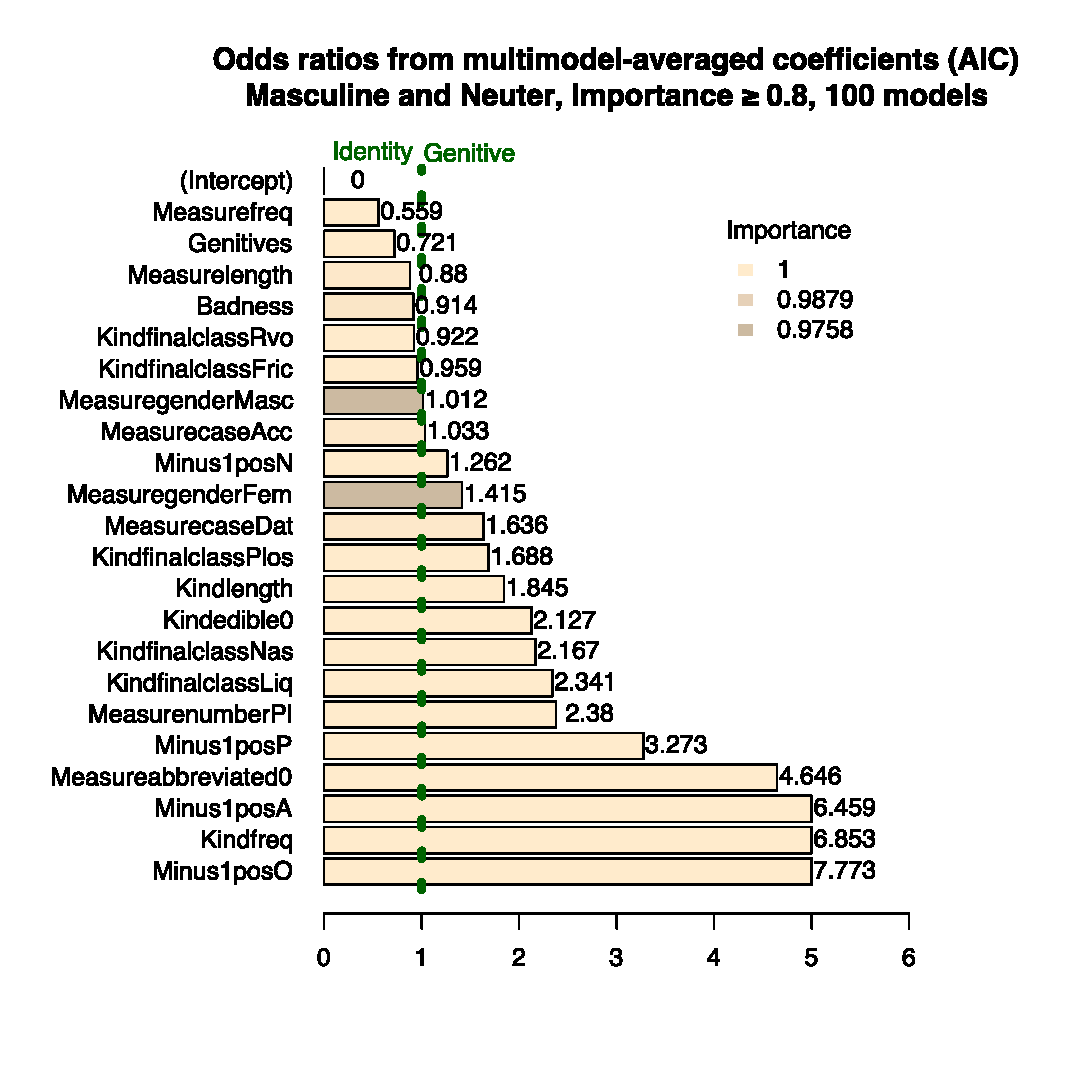
\includegraphics[width=0.5\textwidth]{mn_aic_multi}~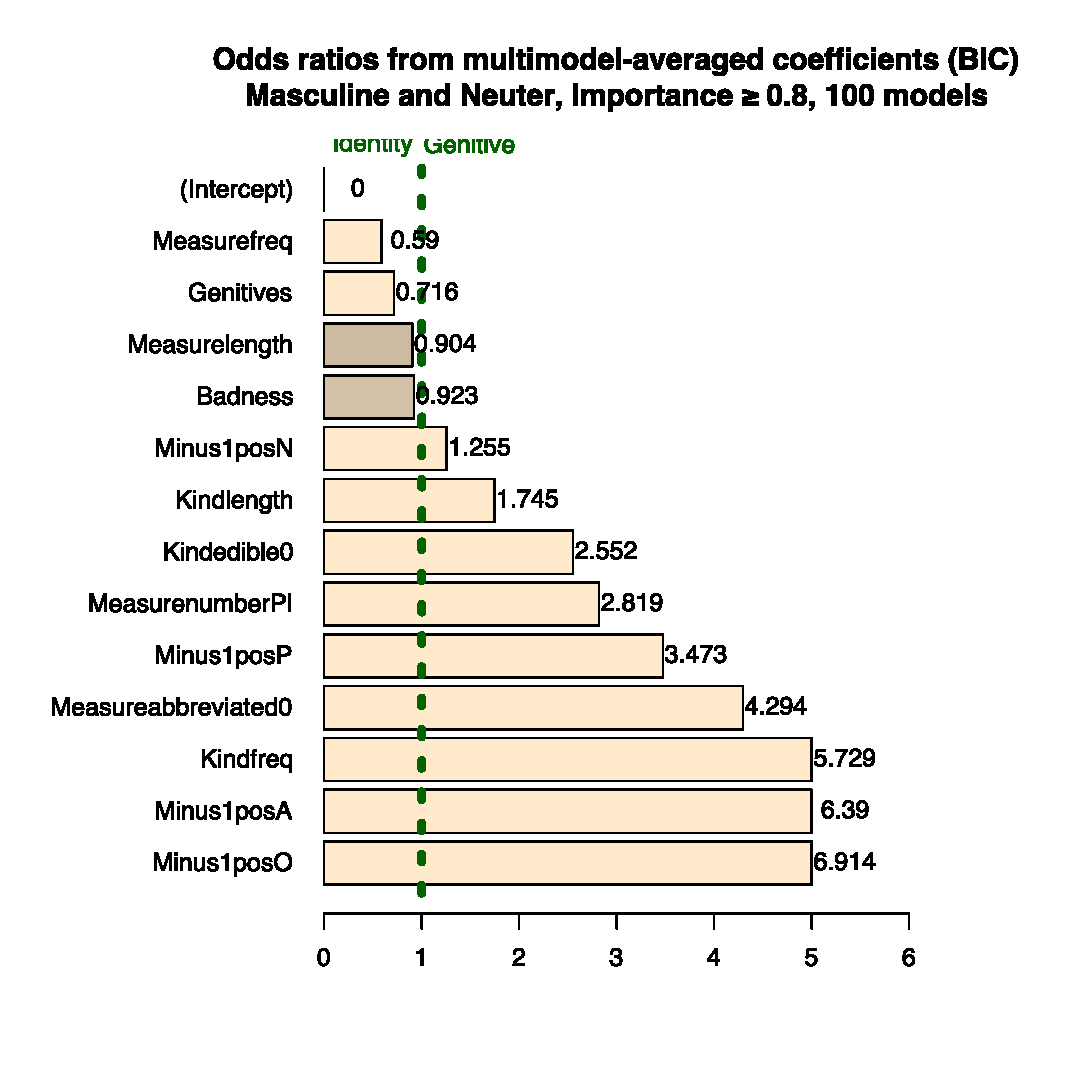
\includegraphics[width=0.51\textwidth]{mn_bic_multi}
%\end{frame}
%
%\begin{frame}
%	{Which IC to use: feminine}
%	\centering
%	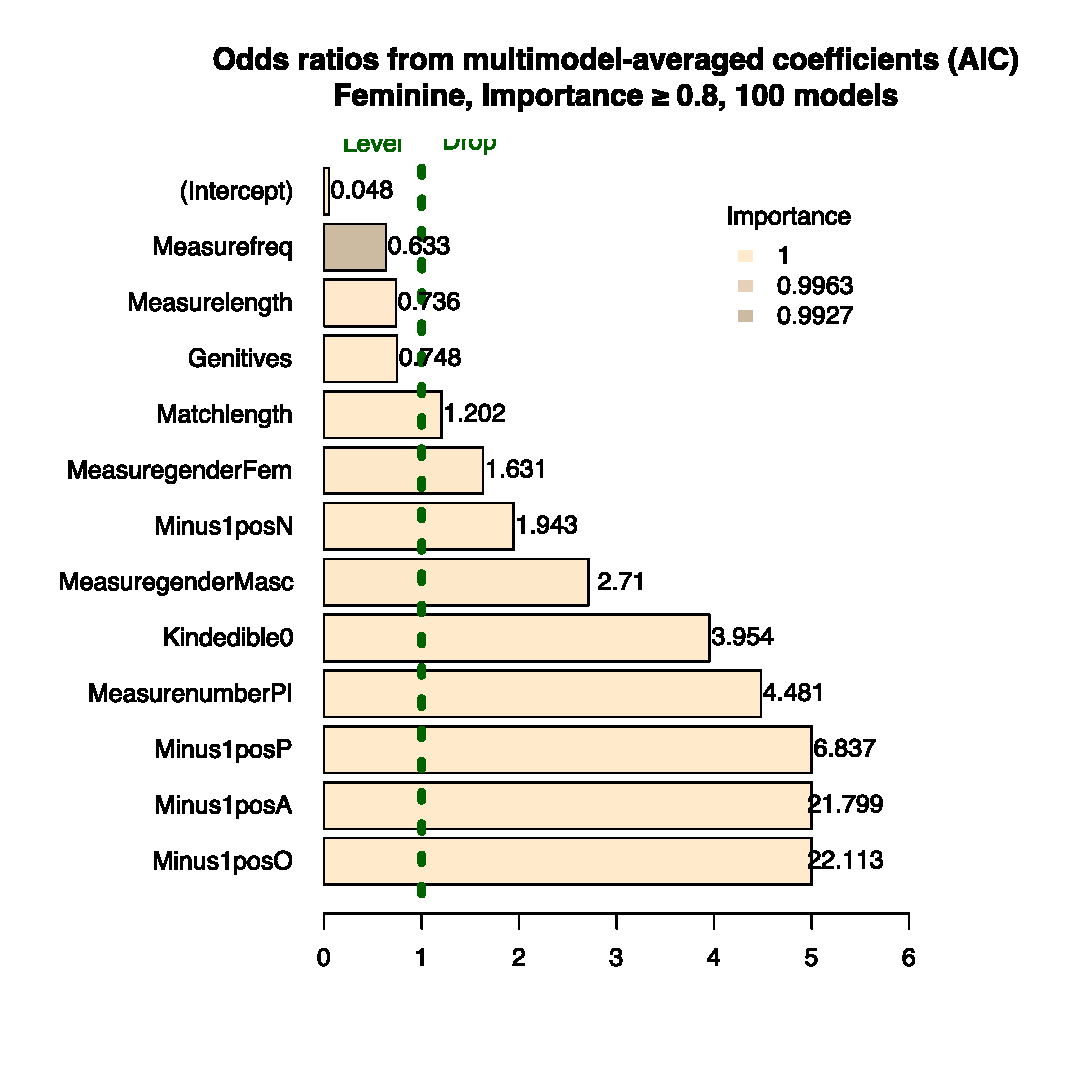
\includegraphics[width=0.5\textwidth]{fem_aic_multi}~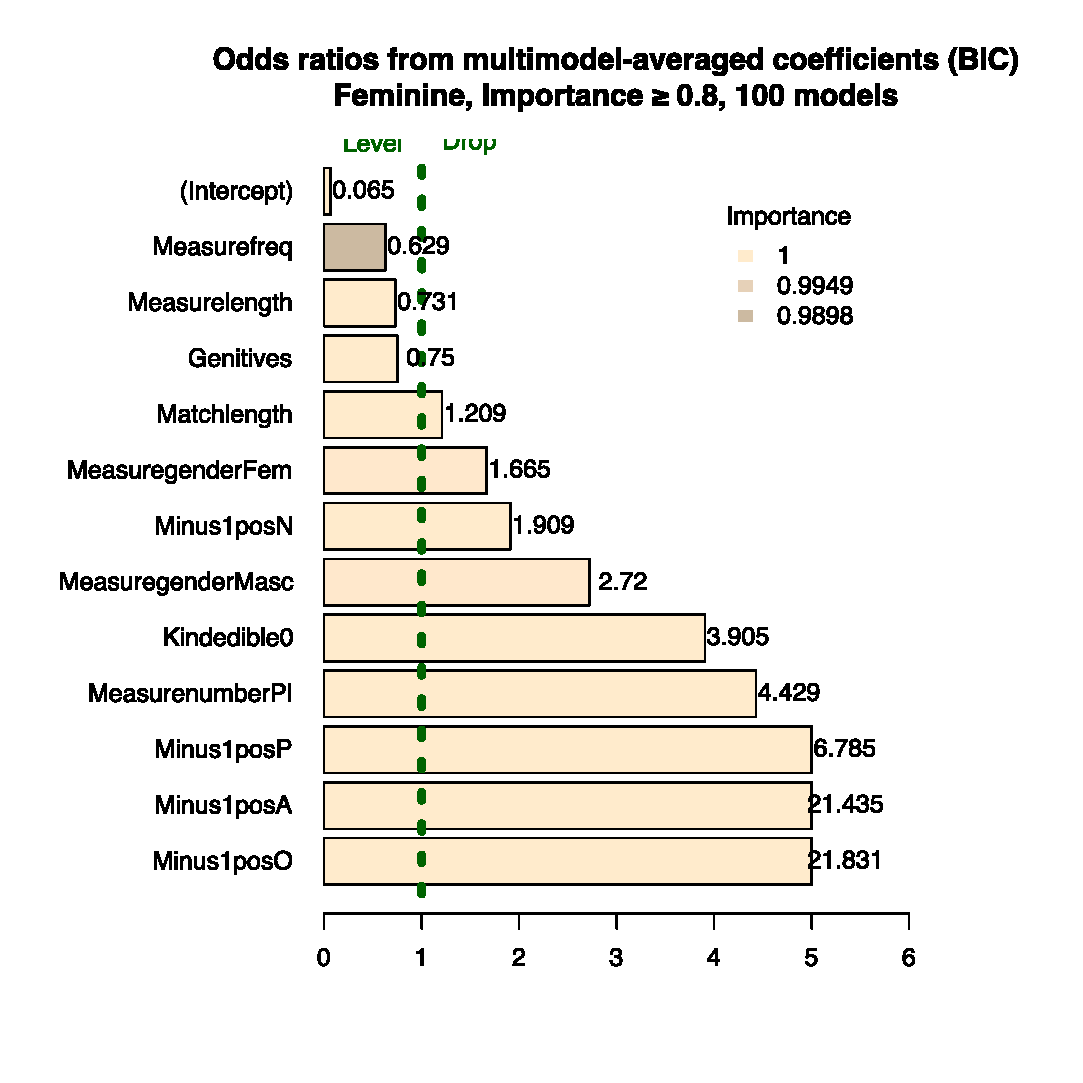
\includegraphics[width=0.51\textwidth]{fem_bic_multi}
%\end{frame}
%
%\begin{frame}
%	{Source of difference between AIC and BIC for masculine}
%	\centering
%	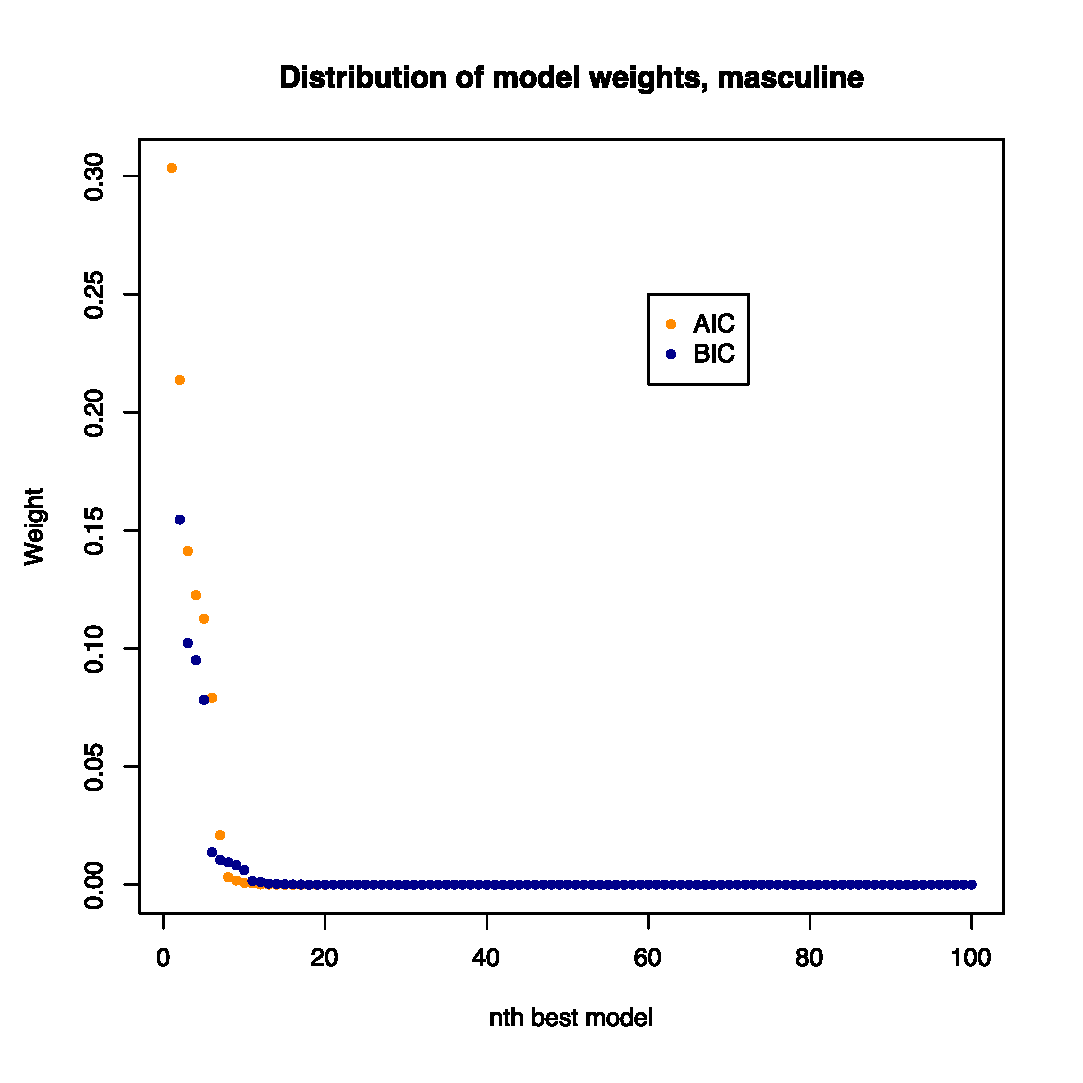
\includegraphics[width=0.5\textwidth]{bic_vs_aic_mn}~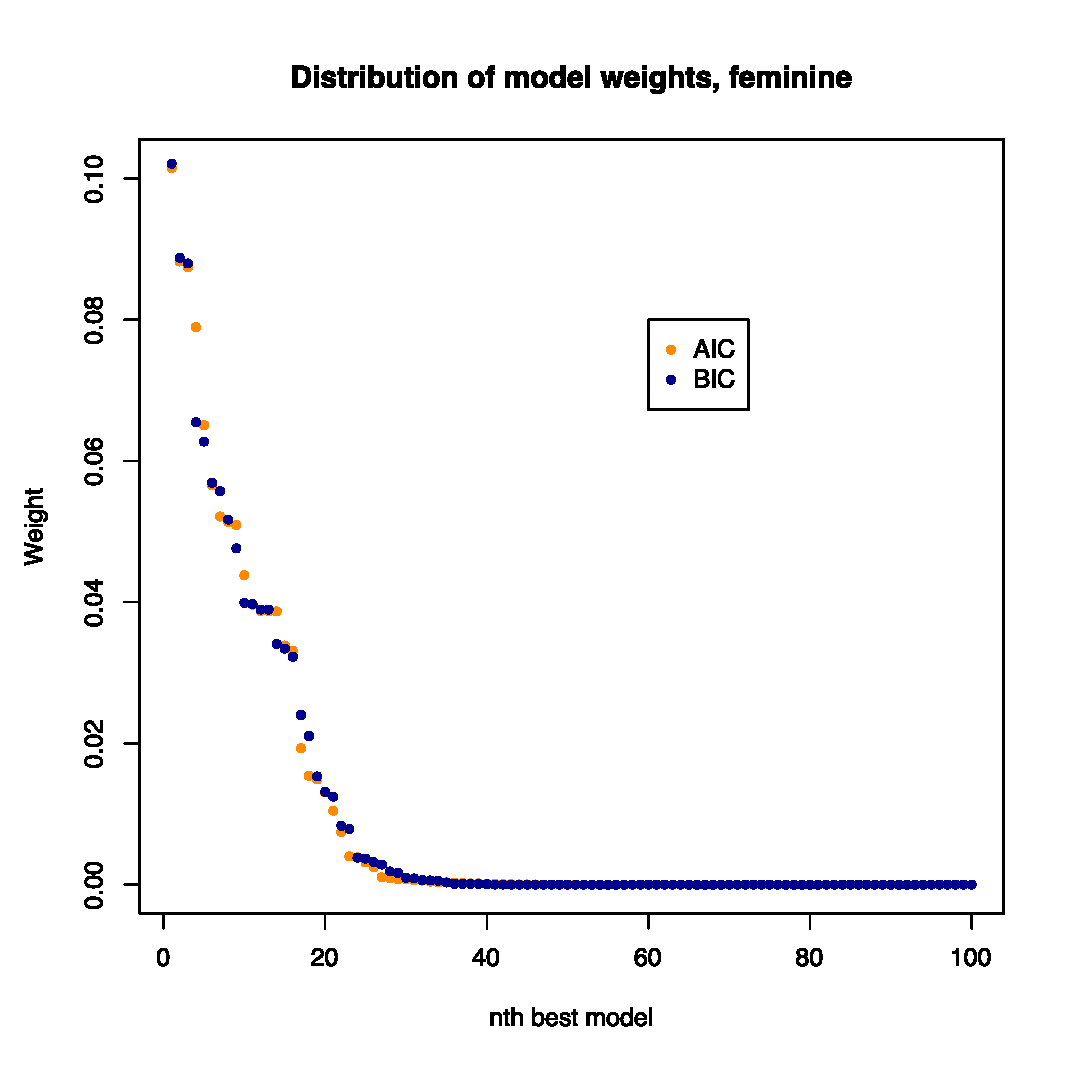
\includegraphics[width=0.5\textwidth]{bic_vs_aic_fem}
%\end{frame}
%

%\subsection{(Preliminary) conclusions and the future}

\begin{frame}
	{Comparison of results}
	\centering
	\scalebox{0.4}{
	\begin{tabular}{lp{0.2cm}cccccp{0.2cm}cccc}
		&& \multicolumn{5}{c}{masc\slash neut} && \multicolumn{4}{c}{fem} \\
		\cline{3-7}\cline{9-12}
		regressor && DEWAC m & DEWAC n & COW & COW AIC & COW BIC && DEWAC & COW & COW AIC & COW BIC \\
		\hline
		\hline
		Badness             &&     &     &     & $-$ & $-$ &&     &     &     &   \\
		\hline
		\alert<2->{Genitives}           &&     &     &     & $-$ & $-$ &&     & $-$ & $-$ & $-$ \\
		\hline
		Kindedible0         &&     &     & $+$ & $+$ & $+$ &&     & $+$ & $+$ & $+$ \\
		\alert<2->{Kindedible1}         &&     &     & $-$ & $-$ & $-$ &&     & $-$ & $-$ & $-$ \\
		\hline
		KindfinalclassFric  &&     &     &     & $-$ &     &&     &     &     &   \\
		KindfinalclassLiq   &&     &     & $+$ & $+$ &     &&     &     &     &   \\
		KindfinalclassNas   &&     &     & $+$ & $+$ &     &&     &     &     &   \\
		KindfinalclassPlos  &&     &     & $+$ & $+$ &     &&     &     &     &   \\
		KindfinalclassRvo   &&     &     &     & $-$ &     &&     &     &     &   \\
		KindfinalclassV     &&     &     & $-$ & $-$ &     &&     &     &     &   \\
		\hline
		\alert<2->{Kindfreq}            && $+$ & $+$ & $+$ & $+$ & $+$ && $+$ &     &     &   \\
		\hline
		Kindlength          &&     &     & $+$ & $+$ & $+$ &&     &     &     &   \\
		\hline
		Matchlength         &&     &     &     &     &     &&     & $+$ & $+$ & $+$ \\
		\hline
		Measureabbreviated0 && $+$ & $+$ & $+$ & $+$ & $+$ && $+$ &     &     &   \\
		\alert<2->{Measureabbreviated1} && $-$ & $-$ & $-$ & $-$ & $-$ && $-$ &     &     &   \\
		\hline
		MeasurecaseAcc      && $-$ & $-$ & $-$ &($+$)&     && $-$ &     &     &   \\
		MeasurecaseNom      && $-$ & $-$ & $-$ & $-$ &     && $-$ &     &     &   \\
		\alert<2->{MeasurecaseDat}      && $+$ & $+$ & $+$ & $+$ &     && $+$ &     &     &   \\
		\hline
		\alert<2->{Measurefreq}         &&     &     & $-$ & $-$ & $-$ &&     &     & $-$ & $-$ \\
		\hline
		MeasuregenderFem    &&     &     & $+$ & $+$ &     &&     & $+$ & $+$ & $+$ \\
		MeasuregenderMasc   &&     &     & $-$ &($+$)&     &&     & $+$ & $+$ & $+$ \\
		MeasuregenderNeut   &&     &     & $-$ & $-$ &     &&     & $-$ & $-$ & $-$ \\
		\hline
		\alert<2->{Measurelength}       &&     &     & $-$ & $-$ & $-$ &&     & $-$ & $-$ & $-$ \\
		\hline
		MeasurenumberSg     &&     &     & $-$ & $-$ & $-$ &&     & $-$ & $-$ & $-$ \\
		\alert<2->{MeasurenumberPl}     &&     &     & $+$ & $+$ & $+$ &&     & $+$ & $+$ & $+$ \\
		\hline
		Minus1posA          &&     &     & $+$ & $+$ & $+$ &&     & $+$ & $+$ & $+$ \\
		\alert<2->{Minus1posC}          &&     &     & $-$ & $-$ & $-$ &&     & $-$ & $-$ & $-$ \\
		Minus1posN          &&     &     &     & $+$ & $+$ &&     &     & $+$ & $+$ \\
		Minus1posO          &&     &     & $+$ & $+$ & $+$ &&     & $+$ & $+$ & $+$ \\
		Minus1posP          &&     &     & $+$ & $+$ & $+$ &&     & $+$ & $+$ & $+$ \\
		\hline
	\end{tabular}
	}
\end{frame}
